\documentclass{article}

\usepackage{arxiv}

\usepackage[utf8]{inputenc} % allow utf-8 input
\usepackage[T1]{fontenc}    % use 8-bit T1 fonts
\usepackage{hyperref}       % hyperlinks
\usepackage{url}            % simple URL typesetting
\usepackage{booktabs}       % professional-quality tables
\usepackage{amsfonts}       % blackboard math symbols
\usepackage{nicefrac}       % compact symbols for 1/2, etc.
\usepackage{microtype}      % microtypography
\usepackage{lipsum}		% Can be removed after putting your text content
\usepackage{graphicx}
\graphicspath{ {./images/} }
\usepackage{doi}

\usepackage[square,numbers]{natbib}

\usepackage{xcolor}
\usepackage{listings}		% code
\definecolor{codegreen}{rgb}{0,0.6,0}
\definecolor{codegray}{rgb}{0.5,0.5,0.5}
\definecolor{codepurple}{rgb}{0.58,0,0.82}
\definecolor{backcolour}{rgb}{0.95,0.95,0.92}

\lstdefinestyle{mystyle}{
    backgroundcolor=\color{backcolour},   
    commentstyle=\color{codegreen},
    keywordstyle=\color{magenta},
    numberstyle=\tiny\color{codegray},
    stringstyle=\color{codepurple},
    basicstyle=\ttfamily\footnotesize,
    breakatwhitespace=false,         
    breaklines=true,                 
    captionpos=b,                    
    keepspaces=true,                 
    numbers=left,                    
    numbersep=5pt,                  
    showspaces=false,                
    showstringspaces=false,
    showtabs=false,                  
    tabsize=2
}

\lstset{style=mystyle}

\title{ZPY: Open Source Synthetic Data for Computer Vision}

\author{
	{\hspace{1mm}Hugo Ponte} \footnote{Correspondence author} \\ 
	Zumo Labs \\
	\texttt{hugo@zumolabs.ai} \\
	\And
	{\hspace{1mm}Norman Ponte} \\
	Zumo Labs \\
	\texttt{norman@zumolabs.ai} \\
	\And
	{\hspace{1mm}Sammie Crowder} \\
	Zumo Labs \\
	\texttt{sammie@zumolabs.ai} \\
	\And
	{\hspace{1mm}Kory Stiger} \\
	Zumo Labs \\
	\texttt{kory@zumolabs.ai} \\
	\And
	{\hspace{1mm}Steven Pecht} \\
	Zumo Labs \\
	\texttt{steven@zumolabs.ai} \\
	\And
	{\hspace{1mm}Michael Stewart} \\
	Zumo Labs \\
	\texttt{michael@zumolabs.ai} \\
	\And
	{\hspace{1mm}Elena Ponte} \\
	Zumo Labs \\
	\texttt{elena@zumolabs.ai} \\
}

% Uncomment to remove the date
\date{\emph{Updated on August 6, 2021}}

\renewcommand{\headeright}{Technical Report}
\renewcommand{\undertitle}{Technical Report}

% PDF metadata
\hypersetup{
pdftitle={ZPY: Open Source Synthetic Data for Computer Vision},
pdfsubject={cs.CV},
pdfauthor={Hugo Ponte, Norman Ponte, Sammie Crowder, Kory Stiger, Steven Pecht, Elena Ponte},
pdfkeywords={Computer Vision, Synthetic Data, Machine Learning, Open Source, Python, Blender},
}

\begin{document}
\maketitle

\begin{abstract}
Synthetic data presents a unique solution to the huge data requirements of computer vision with deep learning. In this work, we present zpy, an open source framework for creating synthetic data in Python. Built on top of the popular open source 3D toolset Blender, zpy is designed with accessibility and readability in mind. Open source synthetic data toolkits like zpy are the bridge between the more mature tools of the 3D workflow and the machine learning frameworks. We make the case for why open source synthetic data is important to solve issues such as fairness and bias by democratizing access to data. Finally, we explore the effect of different types of domain randomization on synthetic training data by fine tuning a CNN on small synthetic training datasets and testing the model on a holdout test dataset of real images. All code is available on GitHub at \url{http://github.com/ZumoLabs/zpy}
\end{abstract}

\keywords{Computer Vision \and Synthetic Data \and Machine Learning \and Open Source \and Python \and Blender}

% https://www.overleaf.com/learn/latex/Inserting_Images
\begin{figure}[!ht]
	\centering
	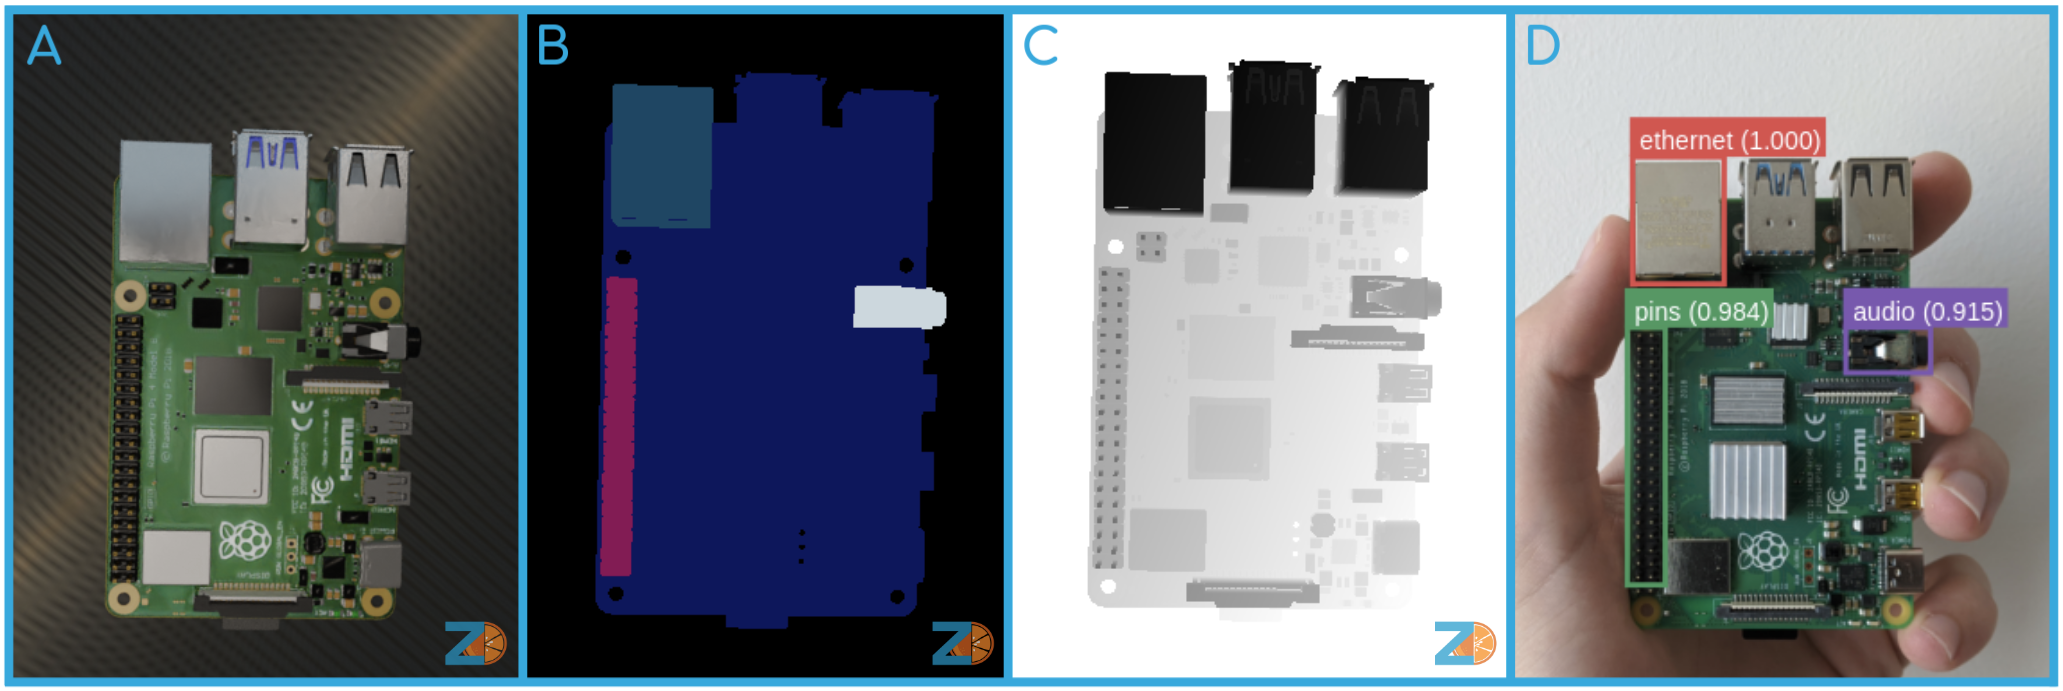
\includegraphics[width=\textwidth]{cover.png}
	\caption{Synthetic images of a Raspberry Pi created with zpy: (A) color image, (B) segmentation image, (C) depth image. These images are used to train a deep learning model, which predicts bounding boxes for circuit board components as seen in the (D) prediction image}
	\label{fig:fig1}
\end{figure}

\section{Introduction}
\label{sec:introduction}

Synthetic data is data that is \emph{created} as opposed to \emph{collected}. Datasets are designed by engineers and researchers such that a statistical learning system trained on this data will behave more predictably and sometimes even perform better. Synthetic data goes beyond curation and allows engineers and researchers to carefully craft the distribution of training data, making sure it has variety in the dimmensions that need it and consistency in other dimmensions.

Simulation heavy fields were amongst the first to start using synthetic images to start training deep learning systems. Research with the biggest datasets and highest quality can be found in these fields, with works on autonomous vehicles \cite{prakash2020structured} \cite{srivastava2019multi} \cite{Hahner_2019} \cite{7780721}, robotic grasping \cite{james2019simtoreal} \cite{tobin2017domain}, and even drone racing \cite{Loquercio_2020}. The availability of high quality 3D humans from the video game and movie industries has also made possible applications such as human pose estimation  \cite{shrivastava2017learning} \cite{Varol_2017}, and person re-id \cite{aaronASRC}. We dive into what synthetic data could mean for human issues such as fairness and bias in \ref{sec:motivation}. Synthetic data has also been used to advance climate and space science, finding applications in detection in overhead satellite imagery \cite{shermeyer2020rareplanes}, pose estimation of satellites in space \cite{kisantal2020satellite}, and segmentation of clouds \cite{lyu2020learning}. Other work has dived deeper into the fundamental theory of synthetic data \cite{le2017using}. For a thorough review of synthetic data literature, we recommend readers go through Nikolenkos 2019 summary paper \cite{nikolenko2019synthetic}.

Analogous to the early days of deep learning, synthetic data still has a black box nature. How to properly create and use synthetic data is not fully understood, and overcoming challenges such as the sim2real gap are still alchemy. We perform an ablation study to examine the effects of domain randomization on synthetic data in \ref{sec:domainrandomization}, and explore the importance of training curriculum in \ref{sec:curicculum}.

Part of the maturation process of deep learning has been the emergence of large open source frameworks such as TensorFlow \cite{tensorflow} and PyTorch \cite{pytorch}. These tools have hundreds of thousands of developers worldwide, and will be the backbone of the AI technologies of the future. As synthetic data itself matures, there too we will see similar open source frameworks emerge. A critical piece of the synthetic data stack, the 3D worfklow, has already produced a champion: Blender \cite{blender}. We study the unique properties of Blender and why it emerged as the frontrunner in the 3D workflow race in \ref{sec:3d}. In fact, zpy is already one of several early attempts at an open source synthetic data toolkit \cite{denninger2019blenderproc} \cite{bpycv}.

\section{Background}
\label{sec:background}

\subsection{3D}
\label{sec:3d}

3D, short for the three dimensions of space we live in, is a catch-all term used to describe the varied technologies used to create virtual worlds. 3D’s technology stack can be roughly split into two broad categories: \emph{asset creation} and \emph{asset scripting}. Asset creation \ref{sec:assetcreation} is the process of creating assets: virtual objects, scenes, and materials. Asset scripting \ref{sec:assetscripting} is the process of manipulating those assets and their interactions over the fourth dimension of time. Decades of progress have resulted in sophisticated software tools that make 3D workflows more automated and straightforward, but a significant amount of human expertise and artistic talent is still required.

\subsubsection{Asset Creation}
\label{sec:assetcreation}

Assets are digital representations of a 3D object. One type of asset is a mesh: a connected graph of 3D points also called vertices, which define the surface of an object. Edges interconnect vertices, and a closed loop of vertices creates a polygon known as a face.

The engineering and manufacturing world creates meshes using computer-aided design (CAD) software such as AutoCAD \cite{autocad}, Solidworks \cite{solidworks}, Onshape \cite{onshape}, and Rhino \cite{rhino}. The entertainment industry creates meshes using modeling software such as Maya \cite{maya}, 3DSMax \cite{3dsmax}, and Cinema4D \cite{cinema4d}.

Whereas a mesh describes the shape and form of an object, a material asset describes the texture and appearance of a virtual object. A material may define rules for the reflectivity, specularity, and metallic-ness of the object as a function of lighting conditions. Shader programs use materials to calculate the exact pixel values to render for each face of a mesh polygon. Modeling software usually comes packaged with tools for the creation and configuration of materials.

Finally, asset creation encompasses the process of scene composition. Assets can be organized into scenes, which may contain other unique virtual objects such as simulated lights and cameras. Deciding where to place assets, especially lights, is still almost entirely done by hand. Automatic scene composition remains a tremendous challenge in the 3D technology stack.

\subsubsection{Asset Scripting}
\label{sec:assetscripting}

The fourth perceivable dimension of our reality is time. Asset scripting is the process of defining the behaviors of assets within scenes over time. One type of asset scripting is called animation, which consists of creating sequential mesh deformations that create the illusion of natural movement. Animation is a tedious manual task because an artist must define almost every frame; expert animators spend decades honing their digital puppeteering skills. Specialized software is often used to automate this task as much as possible, and technologies such as Motion Capture (MoCap) can be used to record the movement of real objects and play those movements back on virtual assets.

Game Engines are software tools that allow for more structured and systematic asset scripting, mostly by providing software interfaces (e.g., code) to control the virtual world. Used extensively in the video game industry after which they were named, examples include Unity \cite{unity3d}, Unreal Engine \cite{unrealengine}, Godot \cite{godot}, and Roblox \cite{roblox}. These game engines support rule-based spawning, animation, and complex interactions between assets in the virtual world. Programming within game engines is a separate skillset to modeling and animating and is usually done by separate engineers within an organization.

\subsubsection{Blender}
\label{sec:blender}

Blender is an open-source 3D software tool initially released in 1994 \cite{blender}. It has grown steadily over the decades and has become one of the most popular 3D tools available, with a massive online community of users. Blender’s strength is in its breadth: it provides simple tools for every part of the 3D workflow, rather than specializing in a narrow slice. Organizations such as game studios have traditionally preferred specialization, having separate engineers using separate tools (such as Maya for modeling and Unreal Engine for scripting). However, the convenience of using a single tool, and the myriad advantages of a single engineer being able to see a project start to finish, make a strong case for Blender as the ultimate winner in the 3D software tools race. 

Many of the world’s new 3D developers opt to get started and build their expertise in Blender for its open-source and community-emphasizing offering. This is an example of a common product flywheel: using a growing community of users to improve a product over time. With big industry support from Google, Amazon, and even Unreal, Blender also has the funding required to improve its tools with this user feedback.

In addition to supporting the full breadth of the 3D workflow, Blender has the unique strength of using Python as the programming language of choice for asset scripting. Python has emerged as the lingua franca for modern deep learning, in part due to the popularity of open-source frameworks such as TensorFlow \cite{tensorflow}, PyTorch \cite{pytorch}, and Scikit-Learn \cite{scikit-learn}. Successful adoption of synthetic data will require Machine Learning Engineers to perform asset scripting, and these engineers will be much more comfortable in Blender’s Python environment than Unity's C\# environment or Unreal Engine’s C++ tools.

\section{Motivation}
\label{sec:motivation}

\subsection{Democratization of Data}
\label{sec:democratizationofdata}

Modern computer vision systems use learning based methods and thus require large and diverse datasets. The need for large and diverse datasets results in a data moat that precludes small companies from competing in the CV market. To amass a good dataset, a company needs time and money: precisely the two things that small nascent companies do not have. 

\subsection{The Status Quo}

The problem lies in how the data pipeline works today. Currently, datasets are almost exclusively collected. mages are stored in databases as they are cumulatively generated by users of a product over time. Annotations are created by hand, usually by a third party provider using low-skilled labor in third world countries. Collecting and labeling a dataset large enough to train a robust computer vision model can take years. Moreover, labeling is not a one-off step, but rather a process that has to be repeated many times. Hand labeled data has shown itself to be imperfect. As one example, studies have found that the widely used ImageNet test set has an estimated label error rate of 5.8\% \cite{dataerrors}. The result is that only companies that have set up the infrastructure to collect and store large datasets, and then the money to subsequently label them, will have the datasets required to train models., Often, the only recourse for a small or newly formed company is to  purchase data from a third party supplier. 


\subsection{Fairness and Bias}

The large cost to collect and annotate datasets makes it prohibitive for most small organizations to create their own datasets, and as such it is common practice to use one of a small selection of openly available datasets (such as ImageNet). This practice has resulted in the pervasive phenomenon of biased algorithms that perpetuate and codify racism, sexism, and bigotry. In the case of human datasets, irresponsibly collected datasets can also raise serious privacy concerns. 

\subsection{Algorithmic Bias}

Algorithmic bias is when an algorithm exhibits a prejudice or inclination for one outcome over another. Because of how openly available datasets have been collected over time, and due to the unequal global distribution of technologies such as cell phone cameras, datasets are often biased. 

Algorithms don’t make fairness; they automate the status quo. The real world is biased and unfair. In human datasets, inevitably, publicly available image datasets exhibit Amero-centric and Euro-centric representation bias and do not adequately address true cultural, demographic, or gender diversity\cite{shankar2017classification}. Widely used public datasets for object recognition also fail to capture all geographic differences\cite{DBLP:journals/corr/abs-1906-02659}. 

Biased datasets result in biased algorithms. The nature of statistical learning methods means that training on these biased datasets will result in a biased model since a model is only as good as the data on which it is trained. The pervasive use of data-driven algorithms has complex social implications: from racial facial recognition \cite{fvrt}, to predictive policing systems that act to confirm and deepen existing biases \cite{predictivepolicing}.

\subsection{Privacy}

Using real data to train models presents very serious privacy risks with the rise of comprehensive privacy regimes like the GDPR in Europe and the CCPA in California. Openly available datasets offer no privacy guarantees as to whether all humans and biometrics represented in the dataset have been acquired with consent. 

Generally, today, the practice when using real datasets is to subject them to a de-identification process. De-identification, sometimes referred to as anonymization, strips a dataset of personal identifiers. However, there are two problems with this process: one, all anonymized data is subject to reversal. The only real bar is the state of technology at the point in time. Anonymized data today becomes pseudonymized data (data that can be reversed and re-identify individuals) tomorrow as models become better at re-identifying data points. Second, anonymized data is not as useful: it is less rich and many times lacks the information required to train a model. 

\subsection{Synthetic Data as a Solution}

Synthetic data can democratize access to large-scale datasets by reducing the time required to collect these datasets and eliminating the cost of labeling these datasets.

Furthermore, synthetic data presents a solution to algorithmic bias: synthetic datasets offer complete control of the distribution and can thus be representatively designed. A synthetic human dataset can be constructed to represent cultural, demographic, and gender diversity equally.  A variety of computer vision domains have explored using synthetic datasets to reduce bias effectively \cite{DBLP:journals/corr/abs-2004-13866}.

Finally, synthetic datasets, by virtue of being created and not collected, guarantees privacy compliance. Synthetic data is free of personal identifiers that could be susceptible to re-identification down the road. Synthetic data guarantees privacy by changing the paradigm and getting rid of any need to use real data.

\begin{figure}
	\centering
	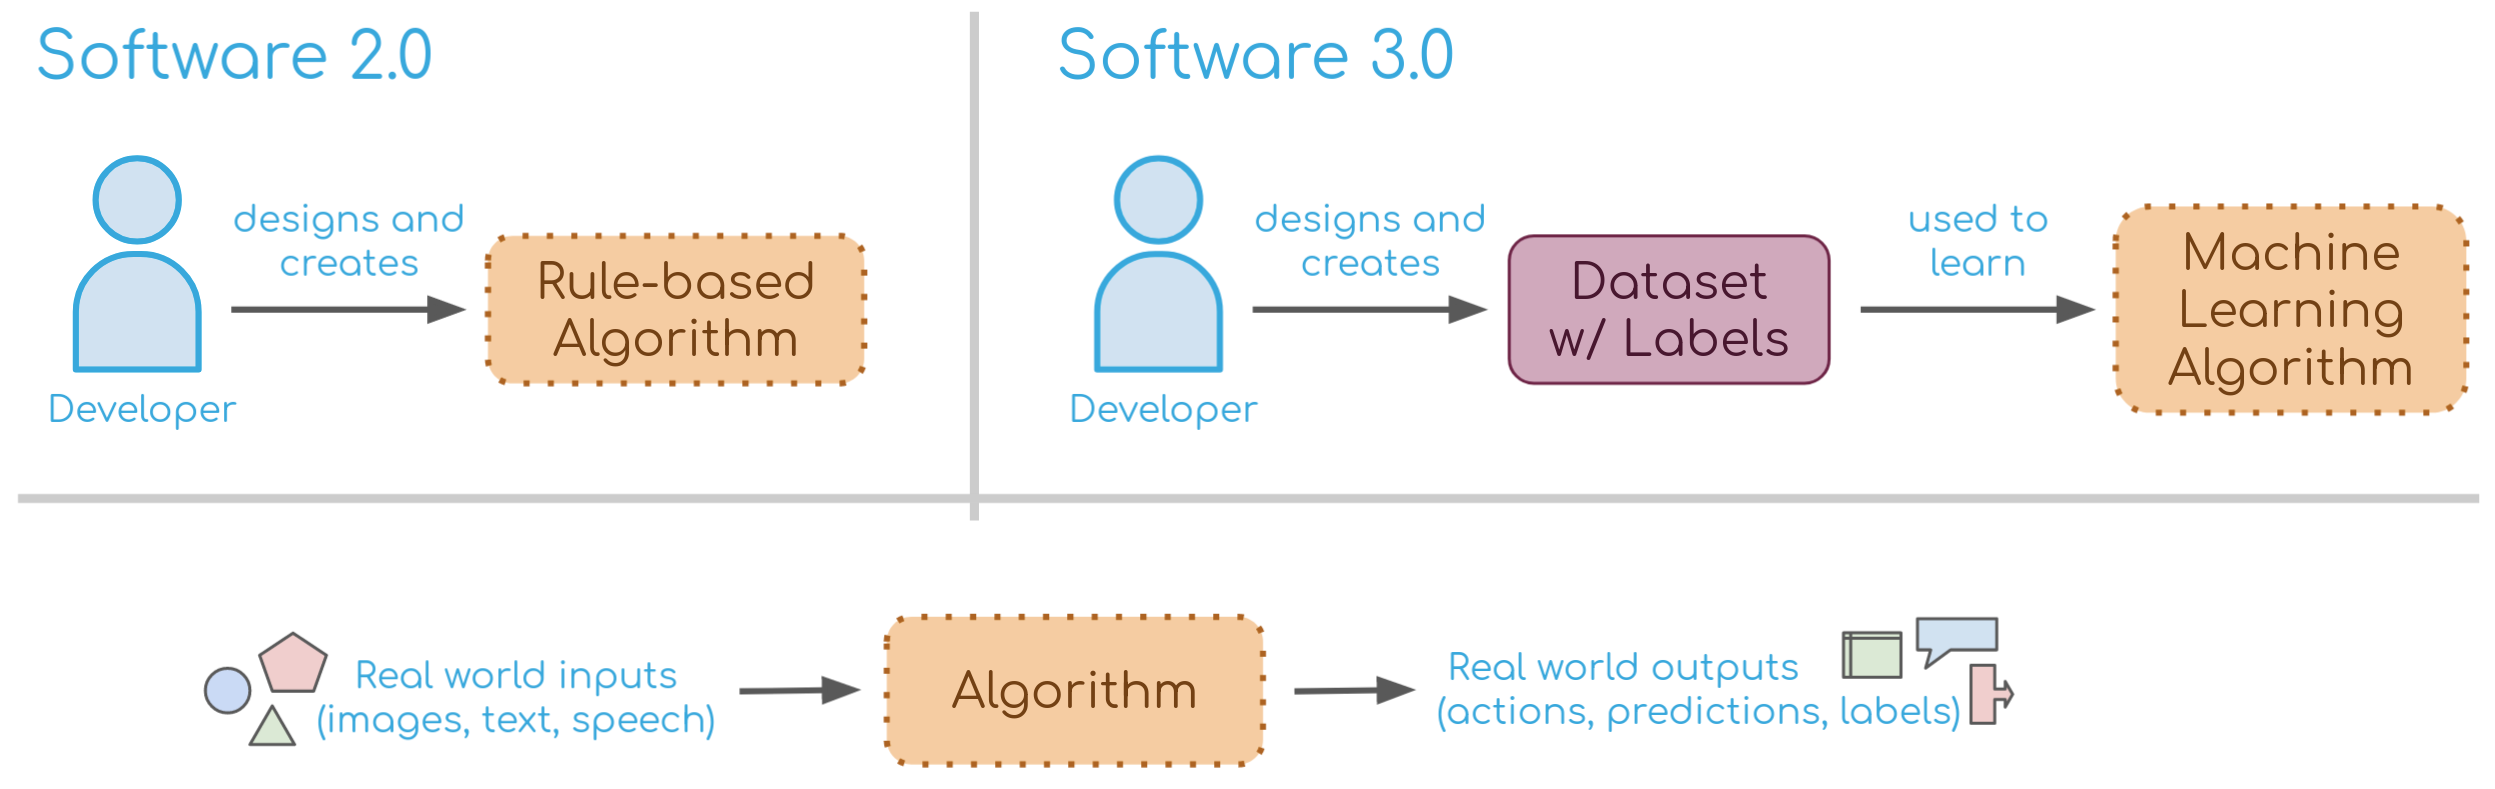
\includegraphics[width=\textwidth]{software3.png}
	\caption{The developer transitions from writing explicit rule-based algorithms (\emph{Software 2.0}) to creating and curating datasets and labels which are used to train machine learning algorithms (\emph{Software 3.0}).}
	\label{fig:fig2}
\end{figure}

\subsection{Software 3.0}
\label{sec:software3.0}

In the software world today, developers write explicit sets of rules also known as algorithms. These algorithms are deployed into production systems, where they consume inputs (i.e. images, text, speech) and produce outputs (i.e. actions, predictions, labels) \ref{fig:fig2}. The relationship between outputs and inputs is carefully managed and designed by developers, and edge cases are identified and bubbled up as exceptions before they can cause unwanted behavior. We nickname this type of explicit heuristic design as \emph{Software 2.0}.

Machine learning based systems, which we nickname \emph{Software 3.0} works differently from these explicitly designed algorithms. Machine learning systems are trained on a dataset, and their behavior in production is often not predictable. Instead of spending their time designing the set of rules that define behavior, or \emph{programming}, we predict the developers of tomorrow will instead spend their time designing a dataset, on which a machine learning system is trained. By designing the dataset, developers will be able to better understand and even make guarantees on the behavior of the machine learning algorithms in production systems. This fundamentally changes the workflow of system development from explicitly writing rules to instead designing datasets, and as such the tools and methods used for programming today will be replaced by dataset design and curation tools.

\section{Project Features}
\label{sec:projectfeatures}

In this section we outline the key features and components of the zpy synthetic data toolkit: a Blender addon \ref{sec:blenderaddon}, a cloud backend \ref{sec:cloudbackend}, a python module \ref{sec:pythonmodule}, and various types of user interfaces \ref{sec:userinterfaces}.

\subsection{Blender Addon}
\label{sec:blenderaddon}

Blender allows for user-created AddOns, and provides tooling for integrating addon functionality with the Blender UI. Examples of popular AddOns are NodeWrangler and Botaniq. NodeWrangler adds simple productivity functionality to the Node System, a method of visual scripting common to 3D tools. Botaniq is a library of tree and plant assets, with a built in scattering method hugely popular due to the complexity of creating grass and trees from scratch. Blender users are comfortable installing and using addons as part of their workflow. The zpy-addon allows for mouse and button based versions of the segmentation, sim run script execution, and sim exporting workflows. Though these actions are possible entirely through python code, providing convenient button versions in a UI makes these processes available to a larger community of 3D artists who are not as comfortable in a code-only environment.

\subsection{Cloud Backend}
\label{sec:cloudbackend}

Computing has traditionally relied on Moore’s Law to increase the power of individual computers. In the past decade the individual compute power of a single computer has not increased significantly, and instead the ability to coordinate a large number of individual computers on a single task has become the method for increasing computation. This type of parallel computing has been democratized through the availability of cloud computing platforms such as AWS, GCP, and Azure. However, these platforms remain difficult for the average developer to use effectively, and domain experts are usually required to take software running on a single computer and scale it across many computers in parallel.

Abstracting away the difficulties of the cloud workflow and providing an intuitive and convenient interface for parallelizing computation is thus important for the synthetic data workflow. Dataset generation jobs can be made with the zpy Python API \ref{lst:api} and CLI \ref{lst:cli} such that many computers are used, thus speeding up the generation job. The Zumo Labs cloud uses orchestration technology, e.g. Kubernetes, to spin up and manage new image generation nodes.

\subsection{Python Module}
\label{sec:pythonmodule}

Python is the most popular programming language for creating and training deep learning systems, which are the primary consumers of synthetic image datasets. The zpy synthetic data toolkit is thus written in python, and is available and installable through the Python Package Index PyPI \ref{lst:pipinstall}.

\begin{lstlisting}[language=bash,caption={Installing the zpy python module.},label={lst:pipinstall}]
pip install zpy-zumo
\end{lstlisting}

When designing software systems, there is usually a tradeoff between \emph{flexibility} and \emph{simplicity}. Simplicity is the ability to perform a task with minimal amount of work and a limited understanding of the software package. Flexibility is the ability to support many different tasks and allow for customization. To balance these two competing objectives, we opted for the principle of \emph{hidden complexity} when designing the zpy python package. One such example is the function calls for random HDRIs and textures: these will default to pre-selected random textures unless a specific path is given. Another manifestation of this design principle is in the flexibility of function arguments: the `zpy.opject.segment()` function call can accept an object directly of type `bpy.types.Object`, but it will also accept the unique string name of that object. These design principles reinforce one of the core principles of Python: \emph{readability}. Python insists on human readable syntax, and does not enforce function and variable type annotations, which makes it quicker to prototype code.


The zpy python package is organized as a collection of separate modules. These modules are separated based on their dependencies and functionality. This makes it easier for end users to add custom functionality, or ignore modules with dependencies they do not want. This type of modular design can be seen in other popular python libraries, such as Matplotlib \cite{Hunter:2007}.

\begin{figure}
	\centering
	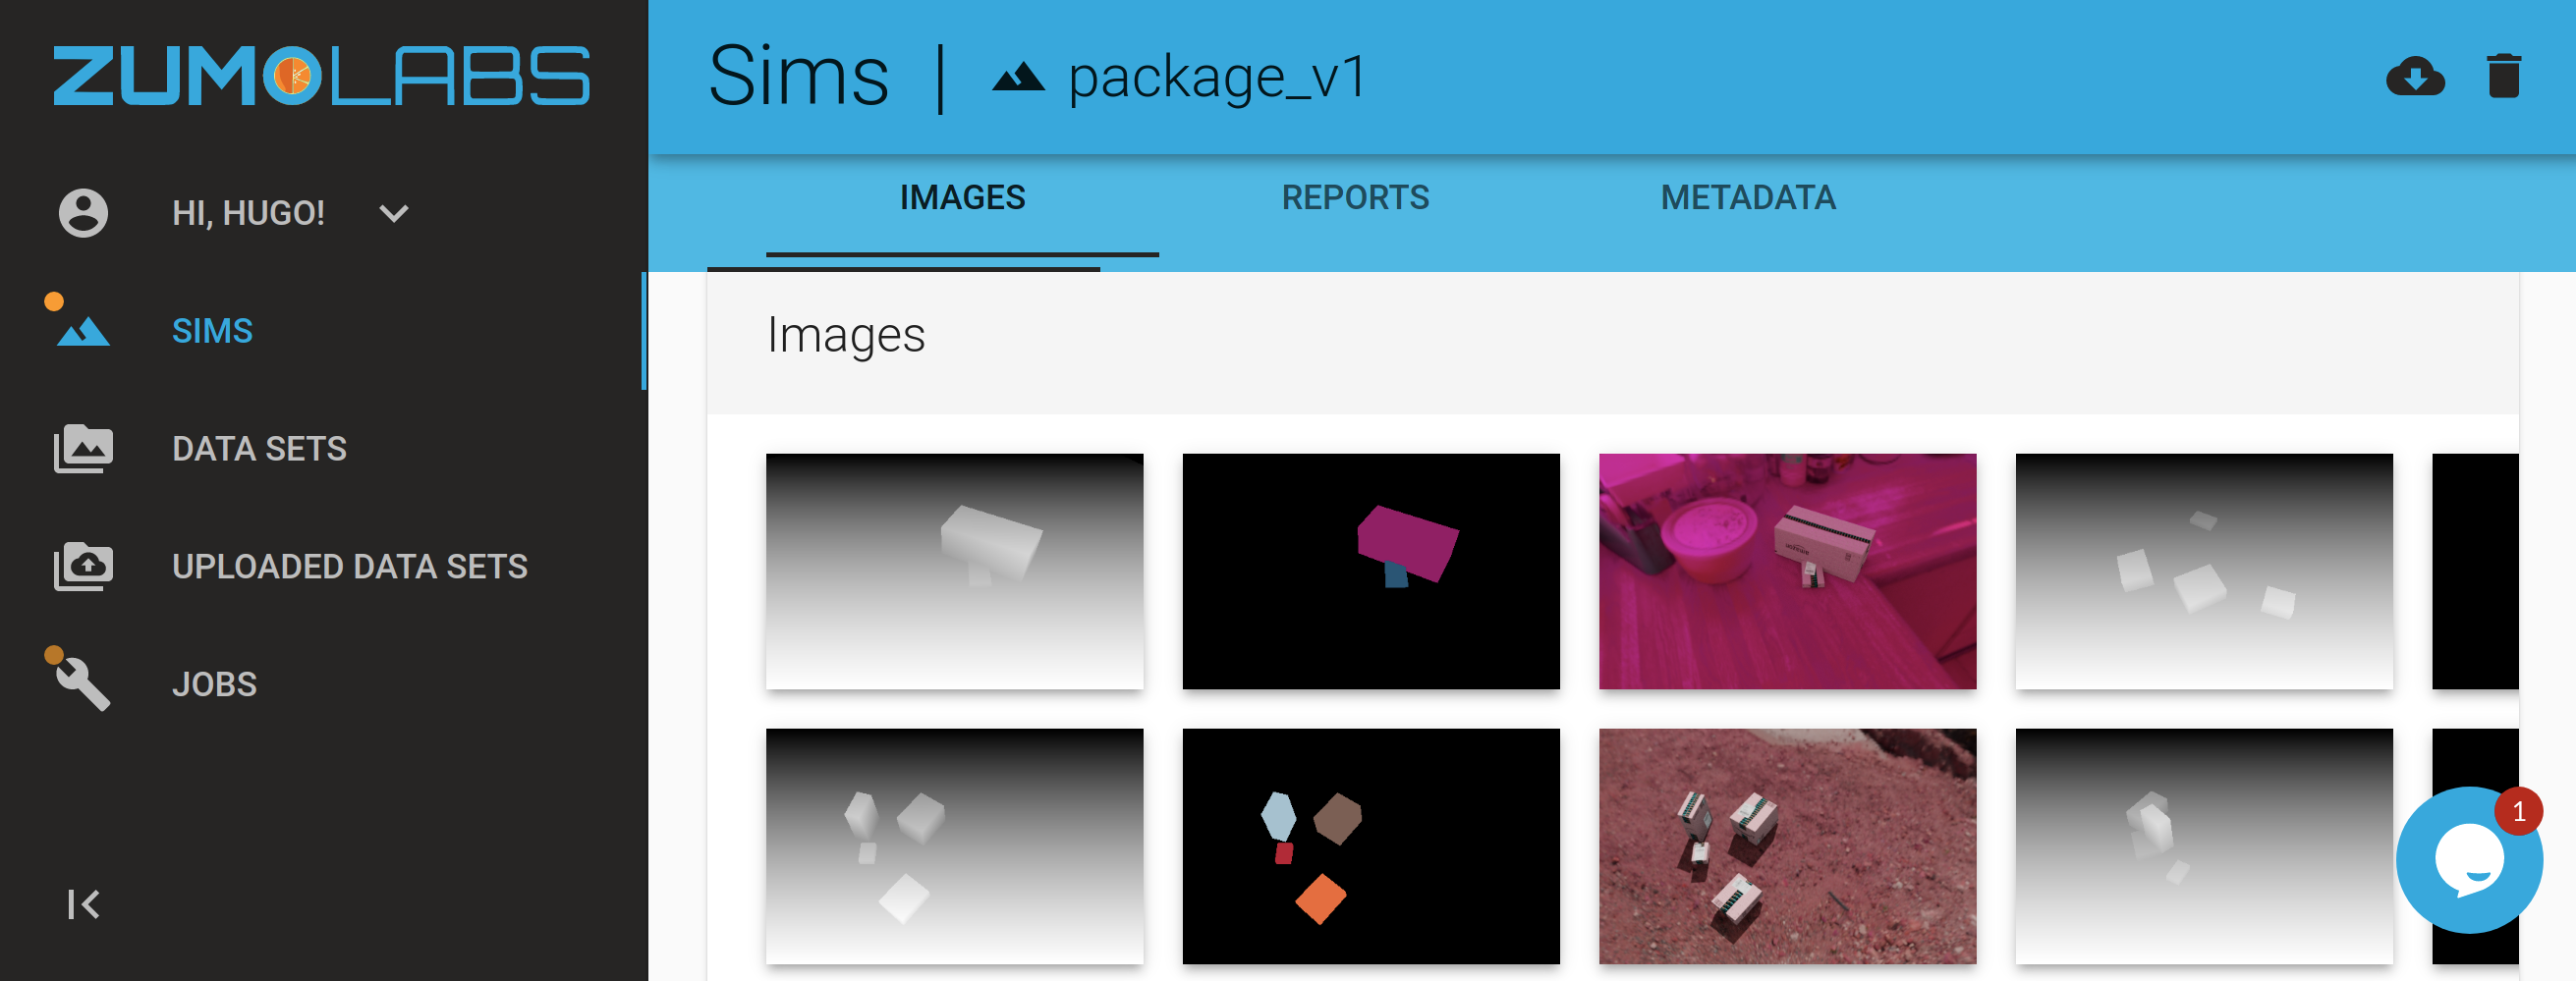
\includegraphics[width=\textwidth]{webapp.png}
	\caption{A visual interface for synthetic data creation via a WebApp.}
	\label{fig:webapp}
\end{figure}

\subsection{User Interfaces}
\label{sec:userinterfaces}

We provide three different interfaces to interact with our product: a Python API \ref{lst:api}, a CLI \ref{lst:cli}, and a graphical WebApp \ref{fig:webapp}. The Python API (application programming interface) allows users to generate custom datasets directly inside a python script, which means that model training code and data generation code can be tied together. This is especially important for using automatic hyperparameter tuning frameworks. The CLI (command line interface) allows for users to generate and manipulate their datasets with unix terminal commands. The terminal is extremely popular as an interface for computation tasks and thus a CLI is a must-have for a large swath of the developer community. Finally, we also provide a graphical interface in the form of a WebApp. Graphical interfaces can provide powerful visualization tools, and are generally more approachable for those less comfortable with code-like interfaces such as an API or CLI. 

\begin{lstlisting}[language=Python,caption={Generating a dataset of 1000 images using the zpy python API.},label={lst:api}]
import zpy
zpy.generate("hello world dataset", 1000)
\end{lstlisting}

\begin{lstlisting}[language=bash,caption={Generating a dataset of 1000 images using the zpy CLI},label={lst:cli}]
zpy create dataset "hello world dataset" my_sim num_images 1000
\end{lstlisting}

\begin{figure}
	\centering
	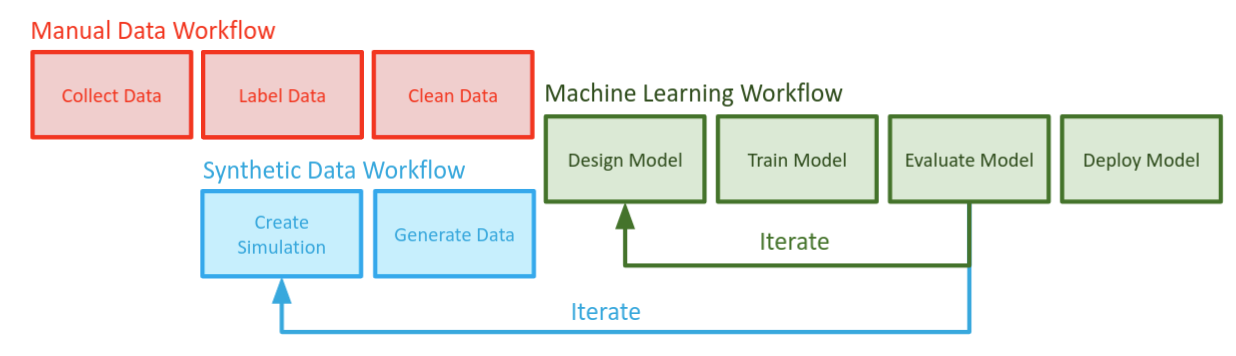
\includegraphics[width=\textwidth]{workflow.png}
	\caption{The synthetic data workflow allows for iteration of the dataset, unlike the manual data workflow, which depends on data collection.}
	\label{fig:workflow}
\end{figure}

\section{Workflow}
\label{sec:workflow}

The full workflow for synthetic data can be reduced into four key steps: \emph{Simulation Creation} \ref{sec:worflowsimcreation}, \emph{Dataset Generation} \ref{sec:generation}, \emph{Model Evaluation} \ref{sec:evaluation}, \emph{Iteration} \ref{sec:iteration}. The synthetic data workflow is similar to the workflow when using collected data, with the key exception that it allows for iteration on the dataset itself \ref{fig:workflow}.

\subsection{Simulation Creation}
\label{sec:worflowsimcreation}

The first step in the syntehtic data workflow is to design and create the \emph{sim}, short for simulation. A sim is a collection of 3D assets controlled at runtime through a single script called the \emph{run script}. The run script defines a function \lstinline{run(**kwargs)}, which acts as the point of entry for any generation process. Important parameters that configure the behavior of the run script are defined as kwargs, short for keyword arguments, in the \lstinline{run(**kwargs)} function. These kwargs allow configuration of the simulation through gin-config, a python package for configuration of python libraries \cite{ginconfig}.

The run script can be broken into two sections: the \emph{setup} and the \emph{loop}. The setup is executed first and typically only once. Setup can include code for creating categories, loading assets, and storing the pose of virtual objects in the scene. The loop, named after the \lstinline{for} loop python pattern, is repeated for some number of frames. Each frame can include code for jittering, saving annotations, and rendering images.

\begin{lstlisting}[language=Python,caption={Basic structure of the run function in a sim run script.},label={lst:setuploop}]
def run(**kwargs):
	# Setup Code
	for frame in zpy.blender.step():
		# Loop Code
\end{lstlisting}


\subsection{Dataset Generation}
\label{sec:generation}

Once a sim has been created it can be used to generate data. There is no constraint on the type of data a sim can generate, though images are the most common. Each frame of the loop in a run script will render out color and segmentation images. Datasets can be generated locally directly inside the Blender GUI through the zpy Blender AddOn \ref{sec:blenderaddon}. This makes sim development possible by making the local debuggin loop faster. Once a sim is properly generating data locally, it can be exported and uploaded to the cloud backend. Exporting is done through the Blender AddOn, and will create a zip file which contains all the asset dependencies required for sim execution. The exported sim can be uploaded to the cloud backend through any of the user interfaces described in \ref{sec:userinterfaces}.

Datasets can be generated in parallel, with multiple cloud machines running concurrent instances of the same sim. Each machine is given a different random seed, resulting in a unique dataset. The resulting collection of smaller datasets can be packaged into into a single larger dataset, making it easier for a machine learning practitioner to download and work with the dataset. Additional workflows are provided for sorting individual datapoints into test, train, and validation buckets.

\subsection{Model Evaluation}
\label{sec:evaluation}

Machine learning models are trained on a dataset for some time, and periodically evaluated on validation and test datasets. Model performance in computer vision can be measured in a variety of ways, such as precision and recall, or more aggregate metrics like mean average precision (mAP). Picking the right metric is problem specific and usually comes down to which type of failure is the most important: false positives or false negatives. It is important to note that though quantitative metrics are convenient, there is no replacement for qualitative analysis of model performance. We recommend that anyone building computer vision models take the time to examine model predictions on real images.

\subsection{Iteration}
\label{sec:iteration}

Those familiar with machine learning model development are aware of \emph{hyperparameters}: parameters whose value are used to control the learning process. Common examples of these include batch size, learning rate, and training epochs. These parameters, unlike the weights inside the model with are learned through training, must be set by the experiment designer. In practice, a human will use their intuition to decide upon a set or range of possible values for these hyperparameters, and then sweep over the possible hyperparameter space to find the best values for a given problem. This process, known as tuning, can have a high cost in engineering time and compute footprint. A technique known as AutoML has improved tuning by significantly reducing the engineering time cost. In AutoML, an automated process will tune these hyperparameters over time by trying different permutations, usually guided through a single heuristic score.

The kwargs of the run function in a sim are effectively additional hyperparameters that can also be tuned. The human designer of the sim can define plausible values and ranges for these sim hyperparameters, and then use an AutoML-like system to discover the values that result in the best model. This presents a unique opportunity in the machine learning workflow, where the dataset used to train a model is no longer static, and can be tuned and improved over time.

\begin{figure}
	\centering
	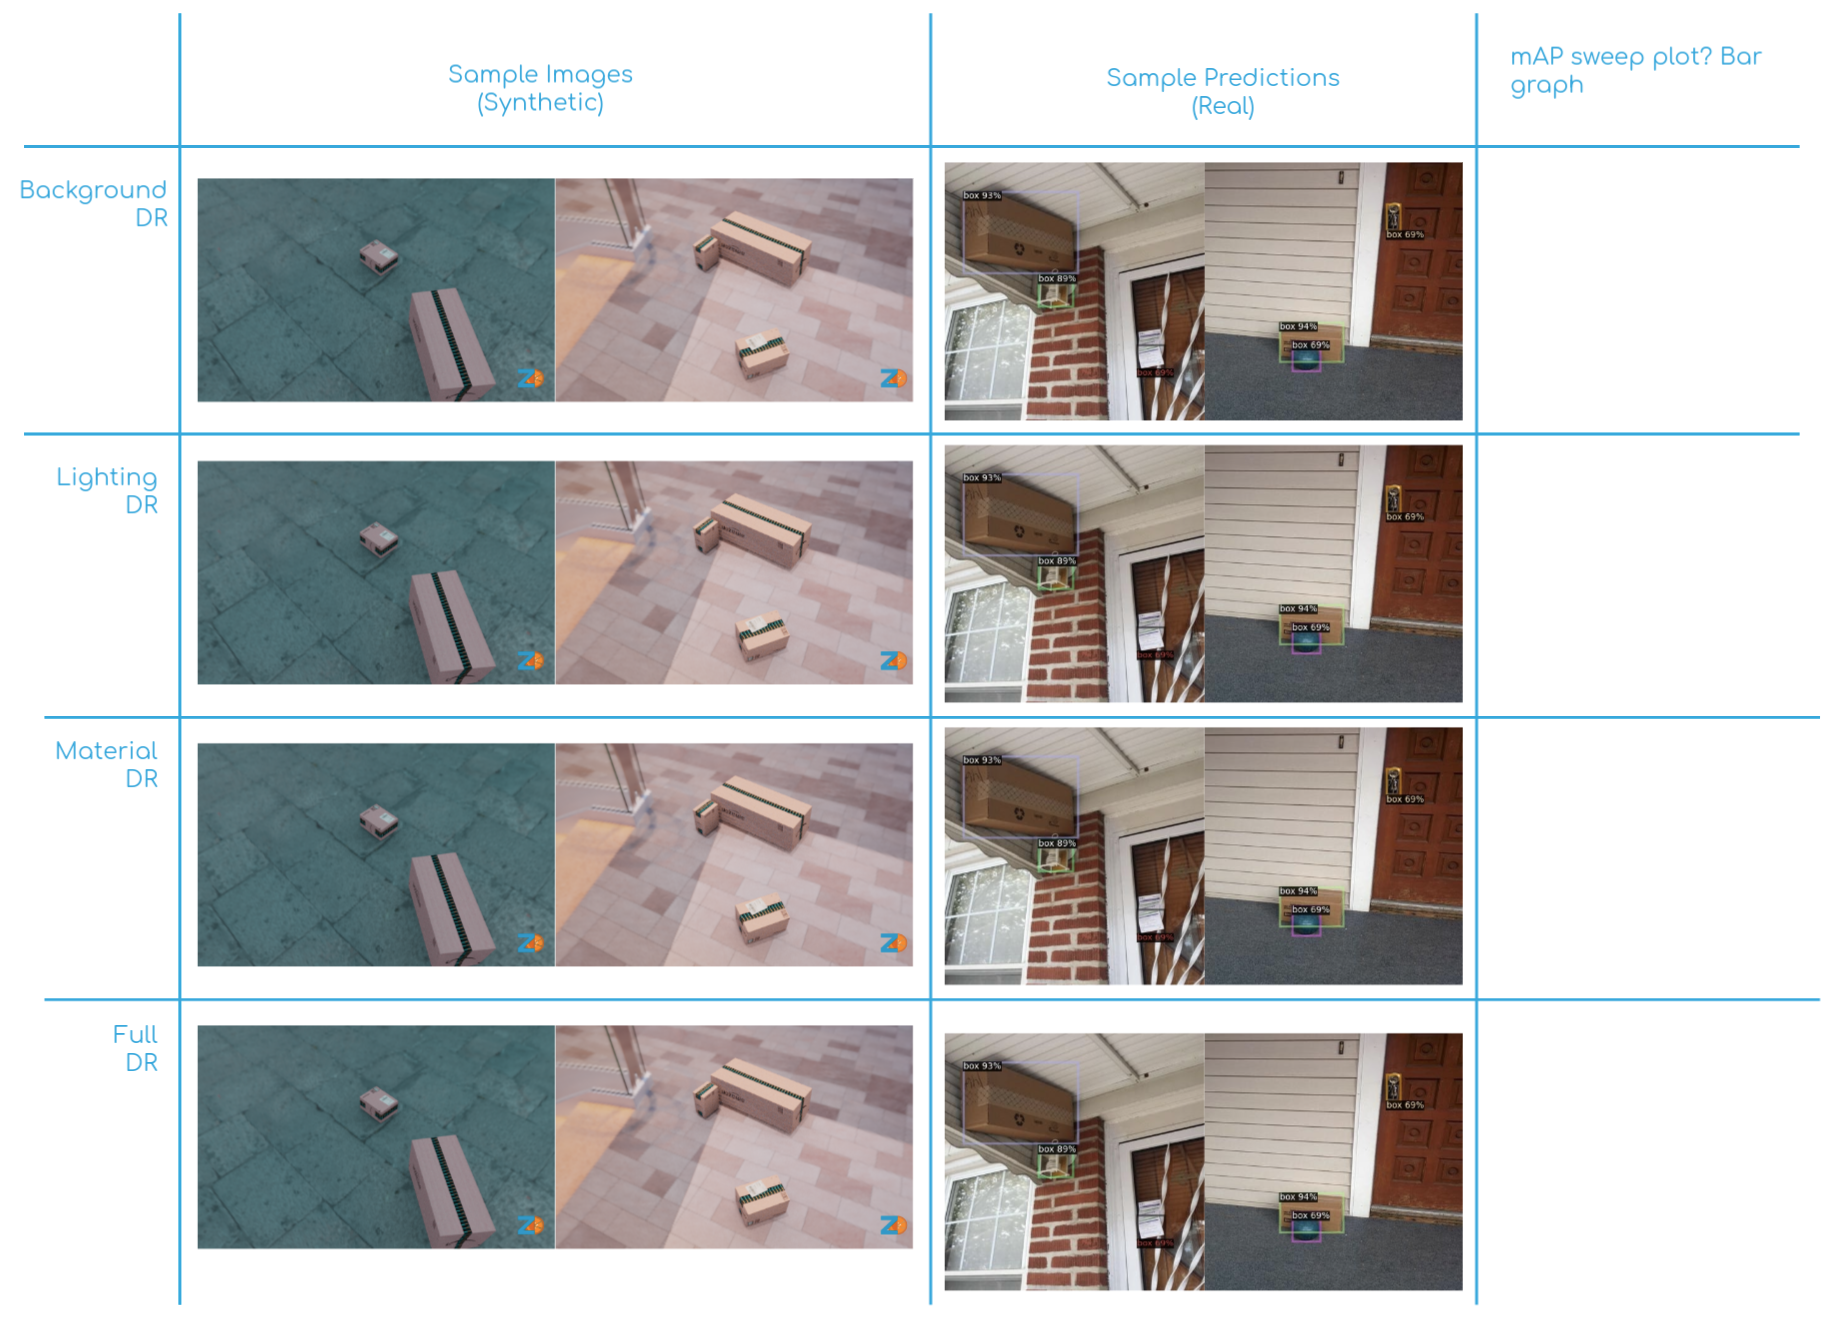
\includegraphics[width=\textwidth]{results.png}
	\caption{(Left) Sample images from synthetic training datasets with different kinds of domain randomization: lighting, background, material, and all of the above. (Right) Bounding box predictions of a model fine-tuned on the corresponding synthetic dataset along with confidence for each detection.}
	\label{fig:results}
\end{figure}

\section{Example}
\label{sec:example}

To put into practice what this paper has explained, we present a simple example of how synthetic data can be used to train a computer vision model. In this example, we train a detection model which predicts the bounding boxes for cardboard packages and parcels in images. In section \ref{sec:trainingmodel} we provide some details on the model and training setup. In section \ref{sec:domainrandomization} we explore how domain randomization in different aspects of the simulation can affect final model performance.

\subsection{Training and Model Specs}
\label{sec:trainingmodel}

We used several variants of Faster R-CNN implemented in PyTorch as part of the Detectron2 model zoo \cite{wu2019detectron2}. Training was done on a single Nvidia GeForce RTX 3090, with each training run lasting at most several thousand iterations, which corresponds to at most 10 epochs given the training dataset size of 512 images. For this experiment we fine-tune a model pre-trained on the COCO detection task as opposed to training the model from scratch. This type of transfer learning is common when using machine learning in the real world due to the quick training speed and relatively good performance. We sweeped over various learning rates and used the largest batch size we could given our GPU memory, model size, and image size. We picked the best performing permutation of hyperparameters when comparing results, using APm on a holdout test dataset of real images.

\subsection{Domain Randomization}
\label{sec:domainrandomization}

Domain randomization is a technique commonly used in synthetic data to increase the variance of a dataset distribution. In the field of synthetic data for computer vision, it might refer to randomizing the intensity of lighting in every frame of a simulation. Domain randomization is also important in the space of material assets: using a large variety of textures and material properties will help prevent texture overfitting, a common issue with CNNs \cite{DBLP:journals/corr/abs-1811-12231}. 

In our package experiment, we expose boolean toggles as run function kwargs that unlock certain forms of domain randomization. One toggle enables domain randomization in the lighting space: changing the position and intensity of several lights in the sim. The second toggle enables random HDRIs, which change the appearance of the background in the package images. The third toggle enables domain randomization for materials, which changes the appearance of the packages themselves, both the texture as well as the material properties. We perform an ablation study to pick appart the contributions of each type of domain randomization to the performance of a detection model trained on synthetic data with each respective form of domain randomization \ref{fig:results}. These toggles are used to create the following four synthetic training datasets:

\begin{itemize}
	\item \lstinline{package_sim_dr_light} - Synthetic dataset of 512 images. Domain randomization is applied to lighting only. The position of a sun light object in the scene, as well as the intensity of the light, is randomized within a range for every image
	\item \lstinline{package_sim_dr_mats} - Synthetic dataset of 512 images. Domain randomization is applied to materials only. The material of each individial package is created in each image, starting with a randomly chosen texture from a library of thousands of textures scraped from the internet. Several properties of the material, such as specular, metallic, and roughness are then jittered within a broad range.
	\item \lstinline{package_sim_dr_bg} - Synthetic dataset of 512 images. Domain randomization is applied to background only. Each image is rendered with a different HDRI, which is chosen from a library of hundreds of HDRIs scraped from the internet.
	\item \lstinline{package_sim_dr_all} - Synthetic dataset of 512 images. Domain randomization is applied to lighting, background, and materials.
\end{itemize}

The best performing single run is fine tuned for 500 iterations at a learning rate of 0.001 on the \lstinline{package_sim_dr_mats} dataset. Comparing the top performing runs for each type of domain randomization, we rank the relative importance of each type: all (46.3 APm), materials (44.9 APm),  lighting (42.1 APm), and background (40.4 APm). One possible explanation for material domain randomization being most important is that the shape of the cardboard box is the more important feature for the model to focus on (as opposed to the material and texture). As a caveat: it is important to underline that this is a small experiment: small models trained for a short amount of time on small datasets. We do not claim that these insights can be applied to other usecases or even further explorations of this particular problem. 

\section{Conclusion}
\label{sec:conclusion}

Synthetic data, data that is \emph{created} as opposed to \emph{collected}, presents a unique solution to the huge data requirements of computer vision with deep learning. The software for the design and creation of synthetic datasets are still primitive, and in this paper we present our attempt at this new type of developer tool: zpy, an open source framework for creating synthetic data in Python. Built on top of the popular open source 3D toolset Blender, zpy is designed with accessibility and readability in mind. Open source synthetic data toolkits like zpy are the bridge between the more mature tools of the 3D workflow and the machine learning frameworks. We make the case for why open source synthetic data is important to solve issues such as fairness and bias by democratizing access to data. Finally, we explore the effect of different types of domain randomization on synthetic training data by fine tuning a CNN on small synthetic training datasets and testing the model on a holdout test dataset of real images. All code is available on GitHub at \url{http://github.com/ZumoLabs/zpy}

\section{Thanks}
\label{sec:thanks}

 Thanks to the developer community of zpy for their feedback and contributions. Thanks to the investors and supporters of Zumo Labs for believing in the future of synthetic data. Thanks to Aaron Dant and his team at ASRC Federal for discussions about synthetic data and comments on this paper.

\bibliographystyle{abbrvnat}
\bibliography{references}

\end{document}


